\ifthenelse{\boolean{acl}}{\section{Multi-participation \blts}}{\section{Optimizing \blts for Multiple Participations}} \label{sec:blt_mp}
We study how to optimize for the BLT parameters $\theta \in \R^d$ and $\omega \in \R^d$ in \cref{eq:blt_noise} for the BLT-DP-FTRL algorithm, and account for DP guarantees. Particularly, we generalize the BLT optimization and DP accounting in \citep{mcmahan2024efficient} from single participation to multiple participations

\subsection{Sensitivity Under Multiple Participations}\label{sec:sensitivity}

\ifthenelse{\boolean{acl}}{
We provide additional background about multi-participation sensitivity definition, computation and usage in DP in \cref{app:mp_sens}, and only discussing the main results in this section. We further derive a lower bound for sensitivity in \cref{app:sens_lower_bound} used for \treeagg in simulation experiments in \cref{sec:exp}.
}{
\paragraph{Adjacent Data Streams and Privacy Accounting} We assume users (FL clients) participate in training according to a \emph{participation schema} $\Pi \subset \text{Powerset}([\nd])$, where each \emph{participation pattern} $\pi \in \Pi$ (and so $\pi \subseteq [\nd]$) indicates a set of indexes of steps in which a single user might participate. 
Each $\Pi$ results in a adjacency relation $\bfN_\Pi$ on data streams:
two data streams $\obs$ and $\obsp$ are adjacent, that is $(\obs, \obsp) \in \bfN$, if there exists a $\pi \in \Pi$ such that $\obs_t = \obsp_t$ for $t \notin \pi$, and $\norm{\obs_t - \obsp_t}_2 \le \clipnorm$ for $t \in \pi$. 
In FL for user-level DP (~\cref{algo:dpfl}), $\obs_t:=\sum_i \Delta_i^t$ is a sum over per-user model gradients each subject to an L2-norm bound $\clipnorm$, and two streaming datasets are adjacent if one can be formed from the other by ``zeroing out'' all the gradient contributions from any one user following Defn.~1.1 of~\citet{kairouz21practical}.  
Under this adjacent relationship, the DP guarantees of MF mechanism in DP-FTRL can be accounted for the release of $\bfC \bfX + \zeta \bfZ$ according \cref{eq:matrixmech}, computing the sensitivity of $\bfC \bfX$ to calibrate with the Gaussian noise $\bfZ$ of zero mean and $\sigma$ standard deviation~\citep{choquette2023amplified}. 

\paragraph{Multi-participation Sensitivity} We consider \bparticipation, where the distance between any two participations is \emph{at least} b and there are at most $\maxpart$ total participations, formally 
\[
  \Pi_{\minsep, \maxpart} = \left\{\pi \subseteq [n]  \mid \abs{\pi} < \maxpart, \{i, j\} \subseteq \pi, i \ne j \Rightarrow |i - j| \ge \minsep\right\}.
\]
This is motivated not only by the applicability to federated learning (as discussed by \citet{choquette2023amplified}, which also formalized this schema), but also because (implicitly) it is the participation schema under which \treeagg was extended to multiple participations by \citet{kairouz21practical}.

Let $\deltaset := \left\{ \obs - \obsp \mid (\obs, \obsp) \in \bfN \right\}$ represent the set of all possible differences between adjacent $\obs,\obsp$. Then, the L2 sensitivity of $\bfC$ under $\bfN$ is given by
\begin{equation}\label{eq:sensgeneral}
\sens_{\bfN}(\bfC) = \sup_{(\obs, \obsp) \in \bfN} \| \bfC \obs - \bfC \obsp \|_F
 = \sup_{\contrib \in \deltaset} \| \bfC\contrib \|_F. 
\end{equation}

In this work, we only consider $\bfC \ge 0$ (elementwise), and so the supremum over $\contrib$ in \cref{eq:sensgeneral} will always be achieved by some $\contrib \ge 0$ (observe each non-zero entry $\contrib_i \in \R^\mdim$ can be chosen arbitrarily from the unit ball of radius $\clipnorm$). The non-negativity also implies $\bfC\tp \bfC \ge 0$, and hence following Corollary~2.1 of \citet{choquette22multiepoch}, we have
\begin{equation} \label{eq:sens}
  \sens_{\bfN_\Pi}(\bfC) = \clipnorm \max_{\pi \in \Pi} \norm{\bfC \ind(\pi)}_2 \qquad \text{when} \qquad \bfC \ge 0. 
\end{equation}
where $\ind(\pi) \in \{0, 1\}^\nd$ is given by $\ind(\pi)_i = 1$ if $i \in \pi$ and $0$ otherwise. Note that $\clipnorm$ simply introduces a linear scaling, and so we can take $\clipnorm=1$ w.l.o.g. both when optimizing mechanisms and when computing \maxloss and \rmsloss.

%\bnote{We might instead work from \citet{choquette2023amplified} Eq. (5) and Prop E.1, which handles the dimensionality easily, rather than directly appealing to Cor. 2.1}


}

\newcommand{\cc}{\mathbf{c}}

\ifthenelse{\boolean{acl}}{}{\paragraph{Multi-participation Sensitivity for \blts}}
Let $\bfC = \LtToep(c) \in \R^\dimdim$ be a lower-triangular Toeplitz matrix defined by the sequence of Toeplitz coefficients $\cc = (c_0, c_1, \dots, c_{\nd-1}) \in \R^\N$ as in \cref{sec:background_blt}. We assume $c_i \ge 0$ and $\cc$ is non-increasing, and consider the sensitivity of $\bfC$. 
Let $\cc_i = \bfC\idx{:}{i}$ be the $i$th column of $\bfC$, so $\cc_0 = \cc$ and generally 
\[
\cc_j = \big(\underbrace{0, 0, \dots, 0}_{\text{$j$ zeros}}, c_0, c_1, \dots c_{n-j-1}\big) \in \R^\nd.
\]

\newcommand{\pistar}{\pi^\star}
\newcommand{\ustar}{\ind(\pistar)}
\newcommand{\ii}{{\tilde{\imath}}}
\newcommand{\kk}{k}

The sensitivity of general Toeplitz matrices with decaying coefficients is recently discussed in \citet[Thm. 2]{kalinin2024banded}, which we restate in \cref{thm:toepminsepsens} with our notation. The participation pattern $\pistar$ simply puts the $\maxpart$ participations as early as possible, with each participation separated by exactly $\minsep$. This sensitivity computation is important for both DP accounting and optimizing for BLT parameters in \cref{sec:opt_blt}. 

\begin{theorem}\label{thm:toepminsepsens}
Given a Toeplitz strategy matrix $\bfC = \LtToep(\cc) \in \R^\dimdim$ with $\cc$ non-increasing and non-negative. Then, $\sens_{\Pi_\minsep}(\bfC)$ can be computed in time $\calO(\maxpart \nd)$  as
\[
  \sens_{\bfN_\Pi}(\bfC) = \norm{\bfC \ustar}_2
\]
where $\pistar$ is given by
\begin{equation}\label{eq:badpi}
\pistar = (0, b, 2b, \dots, (k-1)b).
\end{equation}
\end{theorem}

\ifthenelse{\boolean{acl}}{
}{
\paragraph{A Sensitivity Lower Bound} Inspired by \cref{thm:toepminsepsens}, we state a sensitivity lower bound for general matrix in \cref{rem:senslb}. 
An overly optimistic (instead of commonly worst-case) DP guarantees can be computed for MF mechanism with sensitivity in \cref{rem:senslb}. We \emph{only} use \cref{rem:senslb} for the privacy accounting of baseline binary tree mechanisms in simulation experiments in \cref{sec:exp} as the dynamic programming accounting in \citep{kairouz21practical} is computationally expensive. 
In practice we find the lower-bound of \cref{rem:senslb} is tight for the binary tree matrices we consider; proving this is an interesting open problem.
\begin{rem}\label{rem:senslb}
Letting $\pistar \in \Pi$ as in \cref{eq:badpi}, for any mechanism $\bfC$,
\begin{equation}\label{eq:senslb}
\sens_\Pi(\bfC) \geq \norm{\bfC u(\pistar)}_2 
\end{equation}
is a lower-bound on sensitivity (the actual sensitivity might be higher). While \citet{kairouz21practical} introduced a dynamic program for computing binary-tree sensitivity, it requires some work to extend it to the tree completion trick, and in practice it is expensive to compute. Hence, when evaluating \treeagg approaches, for simplicity we use the lower bound of \cref{eq:senslb}, which can be computed immediately for the tree-completion matrices $\bfC$ used when $\nd$ is not a power of $2$.
\end{rem}


}

\ifthenelse{\boolean{acl}}{\subsection{Analytical Utility as Objective}}{\subsection{Evaluating Matrix Factorization Mechanisms}}\label{sec:mf_obj}

While our end goal is good learning performance (as measured by held-out test set accuracy), we can estimate the utility of a matrix mechanism for DP-FTRL by quantifying the error it introduces into prefix sum estimates. 
The total noise introduced by the DP mechanism into prefix sum estimates in \cref{eq:matrixmech} will be $\bfB \bfZ = \widetilde{\bfA \bfX} - \bfA \bfX$ where $\bfZ \in \R^{\nd \times \mdim}$ is IID Gaussian noise with $\sigma$ determined according to the desired DP guarantee, and $\bfB = \bfA \bfC\inv$. We consider two error metrics based on the standard deviation of the total noise added to the prefix sum estimates.  The \maxerr is the worst-case standard deviation in the estimate of any prefix sum, which can be computed as %
%
{\small %
\[
\maxerrop(\bfB) \coloneqq \max_{i \in [\nd]} \sqrt{\sum_{j \in [\nd]} \bfB_{i,j}^2};
\]
}%
similarly the root-mean-squared error over all iterations $i \in [\nd]$ is %
{\small %
\[
\rmseop(\bfB) \coloneqq 
\sqrt{\sum_{i \in [\nd]} \sum_{j \in [\nd]} \bfB_{i,j}^2 / \nd}.
\]
} %

The standard deviation $\sigma$ of the noise $\bfZ$ must scale linearly in the sensitivity of $\bfC$ to achieve a target DP guarantee, so our final measures of noise account for this: %
{\small %
\begin{align}
\maxlossop(\bfB, \bfC) &\coloneqq \maxerrop(\bfB) \cdot \sens_\Pi(\bfC) \label{eq:maxloss} \\
\rmslossop(\bfB, \bfC) &\coloneqq \rmseop(\bfB) \cdot \sens_\Pi(\bfC) \label{eq:rmsloss}
\end{align}
}%
\cref{eq:maxloss,eq:rmsloss} measure the distribution of noise to approximate the privacy-utility trade-off as the loss, which do not depend on the noise multiplier $\alpha=\sigma/\sens_\Pi(\bfC)$ that is directly used in accounting for the DP guarantees, as discussed in \citep[Introduction]{mcmahan2024efficient}. For optimized $\bfC$ in matrix factorization mechanisms (e.g., \treeagg, \bandmf, and \blt), specific DP guarantees are achieved by scaling $\alpha$ (and corresponding $\sigma$ in \cref{algo:dpfl}). The total noise on the prefix sum $BZ$ also scales \maxloss and \rmsloss by $\alpha$. Hence, without loss of generality, we use \rmsloss and \maxloss to compare the optimality of different matrix factorization mechanisms, which is equivalent to assuming $\alpha=1$ that corresponds to $(\epsilon=5.3, \delta=10^{-7})$-DP (for example).
% print(
%    dp_accounting.pld.PLDAccountant()
%    .compose(dp_accounting.GaussianDpEvent(1.0), 1)
%    .get_epsilon(target_delta=1e-7)
%)

Note we deviate from the definitions of \citep[arXiv v3]{mcmahan2024efficient}, in order to distinguish the error introduced by $\bfB$ from the total loss (which is what we optimize and use to compare mechanisms), which incorporates the sensitivity of $\bfC$. 


\ifthenelse{\boolean{acl}}{\subsection{Optimizing Multi-participation \blts}}{\subsection{Optimizing \blts for Multiple Participations}} \label{sec:opt_blt}

\ifthenelse{\boolean{acl}}{}{\begin{algorithm}[htbp]
\caption{Differentiable Loss for BLTs} \label{alg:blt_loss}
\begin{algorithmic}%[1]
\STATE \textbf{Inputs:} 
\STATE \myind Pair of buffer-decay parameters $(\theta, \hth)$ with $\nbuf$ buffers each ($\theta, \hth \in [0, 1]^\nbuf$).
\STATE \myind num rounds $\nd$, min-separation $\minsep$, max participations $\maxpart$
\STATE \myind Penalty strength $\lambda$, set to zero for loss calculation, or $\lambda = 10^{-7}$ to stabilize optimization
\STATE \textbf{Outputs:}

\STATE \myind Either $\maxlossop(\bfA \bfC\inv, \bfC)$ or $\rmslossop(\bfA \bfC\inv, \bfC)$.
\STATE
\STATEComment Use \cref{alg:blt_pair} to calculate the unique $\omega$ and $\homega$ such that $\bfC = \bltm(\theta, \omega)$ and $\bfC\inv = \bltm(\hth, \homega)$
\STATE $\omega = \mathtt{calc\_output\_scale}(\theta, \hth)$
\STATE $\homega = \mathtt{calc\_output\_scale}(\hth, \theta)$
\STATE
\STATEComment Compute $\var{sens} = \norm{\bfC \pistar}_2$ where $\bfC = \LtToep(c)$ 
\STATE Compute $c \in \R^n$ where $c_0 = 1$ and $
c_i = \sum_{j \in [\nbuf]} \omega_j \theta_j^{i-1}$ for $i \in \{1, \dots, \nd\}.$
\STATE $\bar{c} = 0 \in \R^\nd$  \Comment Holds the sum of columns of $\bfC$
\FOR{$i \in [\maxpart]$}
  \STATE $\bar{c}{[b\cdot i:]}\  +\!\!=\  c{[0 : n - b\cdot i]}$  \Comment \texttt{numpy}-like semantics
\ENDFOR
\STATE $\var{sens} = \norm{\bar{c}}_2$ \Comment{Because $\bar{c} = \bfC \pistar$.}
\STATE
\STATEComment Compute $\text{Errror}(\bfA \bfC\inv)$ where $\bfC\inv = \LtToep(\hc)$.
\STATE Compute $\hc \in \R^n$ where $\hc_0 = 1$ and $
\hc_i = \sum_{j \in [\nbuf]} \homega_j \hth_j^{i-1}$ for $i \in \{1, \dots, \nd\}.$
\STATE Compute $b \in \R^n$ by $b_i = \sum_{j=0}^{i} \hc_i$  \Comment So $\bfB = \bfA\bfC\inv = \LtToep(b)$.
\STATE $\var{err} = \begin{cases}
\sqrt{\sum_{i \in [\nd]} b_i^2} & \text{for \maxerr} \\
\sqrt{ \sum_{i \in [\nd]} (n - i) b_i^2 / \nd} & \text{for \rmse}.
\end{cases}$

\STATE
\STATEComment Log-barrier penalties to keep $\theta > 0$, $\theta < 1$, and $\omega > 0$ for numerical stability when optimizing
\STATE $\var{penalty} = \lambda (-\log(\theta) -\log(1 - \theta) -\log(\omega))$

\STATE 
\STATE \textbf{Return} $\var{loss} = \var{err} \cdot \var{sens} + \var{penalty}$
\end{algorithmic}
\end{algorithm}

\begin{algorithm}[htbp]
\caption{\texttt{calc\_output\_scale}  (Lemma 5.2 of \citet{mcmahan2024efficient})} \label{alg:blt_pair}
\begin{algorithmic}%[1]
\STATE \textbf{Input:} 
\STATE \myind Pair of buffer-decay parameters $(\theta, \hth)$ with $\nbuf$ buffers each ($\theta, \hth \in [0, 1]^\nbuf$).

\STATE \textbf{Output:}
\STATE \myind The unique $\omega$ s.t. $\bfC = \bltm(\theta, \omega)$ has a \blt inverse with buffer-decay $\hth$ ($\bfC\inv = \bltm(\hth, \cdot)$).
\STATE
\STATEComment Note that in \citep{mcmahan2024efficient}, $\bfC$ was parameterized by $\hth$ and $\bfC\inv$ was parameterized by $\theta$.
\STATE $p(x) = \prod_{i \in [\nbuf]} (1 - \hth_i x)$
\STATE $q(x) = \prod_{i \in [\nbuf]} (1 - \theta_i x)$
\STATE $f(x) = (p(x) - q(x)) / x$  \Comment Polynomial division gives $f$, a polynomial of degree $\nbuf-1$
\STATE $z = \prod_{i \in [\nbuf]} -\theta_i$ 
\STATE $w_i = \left(\prod_{j \ne i} (\theta_i\inv - \theta_j\inv)\right)\inv$ for $i \in [\nbuf]$
\STATE Define $\omega$ by $\omega_i = f(\theta_i\inv)\frac{-\theta_i w_i}{z}$ for $i \in [\nbuf]$
\STATE \textbf{Return} $\omega$

\end{algorithmic}
\end{algorithm}}

For the typical scale of $\nd < 10^5$ in FL systems, rather than deriving closed forms for sensitivity and error as in \citet{mcmahan2024efficient}, we use an alternative approach that is flexible and simple to implement. 
Recall the properties of BLTs discussed in \cref{sec:background_blt}, we parameterize the optimization of the \blt by the pair $(\theta, \hth)$.  \citet[Lem. 5.2]{mcmahan2024efficient} implies given a pair $(\theta, \hth)$, there exist unique $(\omega, \homega)$ such the $\bltm(\theta, \omega)\inv = \bltm(\hth, \homega)$, and we can compute $\omega$ and $\homega$ in time $\calO(\nbuf^2)$; this result is summarized below as \cref{alg:blt_pair}. Thus, given a $(\hth, \theta)$, we can efficiently compute the Toeplitz coefficients of $\bfC$ (using \cref{eq:closedcoefs} applied to $(\theta, \omega)$) and $\bfC\inv$ (applying \cref{eq:closedcoefs} to $(\hth, \homega)$). From the Toeplitz coefficients of $\bfC$ we can then efficiently compute sensitivity using \cref{thm:toepminsepsens}. \rmse can be computed efficiently from the Toepltiz coefficients of $\bfC\inv$ following the approach of \citet[Prop. 3.1] {mckenna2024scaling}, and a simple generalization of this approach applies to to \maxerr as well. For completeness we summarize in the following proposition:

\begin{prop}\label{prop:toeperror}
Let $\bfC = \LtToep(c) \in \R^\dimdim$ be a lower-triangular Toeplitz matrix defined by Toeplitz coefficients $\cc = (c_0, c_1, \dots, c_{\nd-1}) \in \R^\N$. Then $\bfC\inv$ is also a lower-triangular toeplitz matrix; let $\bfC\inv = \LtToep(\hc)$. Then, $\bfB \coloneqq \bfA \bfC\inv = \LtToep(b)$ where $b_i = \sum_{j=0}^{i-1} \hc_i$. Further, we can compute 
{\small \[ 
\maxerrop(\bfB) 
= \sqrt{\sum_{i \in [\nd]} b_i^2}
\]}%%
and
{\small \[ 
\rmseop(\bfB) 
= \sqrt{ \sum_{i \in [\nd]} (n - i) b_i^2 / \nd}.
\]}%%

\end{prop}

\ifthenelse{\boolean{acl}}{}{
\begin{table*}[htbp]
  \begin{varwidth}[b]{0.54\linewidth}
    \centering
    \begin{tabular}{rrrr}
    \toprule
    $n$ & brute force & via \cref{alg:blt_pair} & speedup \\
    \midrule
    % Computed here: https://colab.corp.google.com/drive/1_BRrt0jUniaOixKwasKDr7jiSToRwJLj#scrollTo=8tnK5aOnESuk
    2000 & 0.021 & 3.8e-5 & 550$\times$ \\
    20000 & 0.258 & 3.6e-5 & 7176$\times$ \\
    200000 & 4.772 & 4.5e-5 & 104884$\times$ \\
    \bottomrule
    \end{tabular}
    \caption{Seconds to compute $n$ Toeplitz coefficients of $\bfC\inv$. JAX just-in-time (JIT) compilation is \emph{not} included for either approach.}    
    \label{tab:c_inv_coef}
  \end{varwidth} %
  \hfill
  \begin{minipage}[t]{0.44\linewidth}
    \centering
    % Source: https://colab.corp.google.com/drive/1_BRrt0jUniaOixKwasKDr7jiSToRwJLj#scrollTo=e6QNruh2_tBz&uniqifier=1
    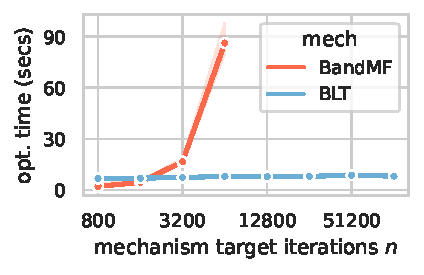
\includegraphics{images/opt_time.pdf} %
    \captionof{figure}{Total wall clock optimization time including JIT compilation on a V100 GPU for \bandmf and \blts, fixing $\minsep=400$ and varying $\nd$. The average over 3 runs is reported.}
    \label{fig:faster}
  \end{minipage}%
\end{table*}


Combining these elements gives us an efficient and differentiable algorithm for computing \maxloss and \rmsloss. Complete pseudo-code for the differentiable loss calculation is given in \cref{alg:blt_loss}. Following \citet{mcmahan2024efficient}, we use auto differentiation and L-BFGS optimizer in JAX~\citep{jax2018github} to optimize $(\theta, \hth)$ for the BLT-DP-FTRL algorithm, and then extract $\bltm(\theta, \omega)$ for noise generation. Similar to \citep{mcmahan2024efficient}, we introduce log-barrier penalties w/ strength $10^{-7}$ to keep $\omega > 0$, $\theta > 0$ and $\theta < 1$ (which is necessary to ensure the Toeplitz coefficients of $\bfC$ are decreasing to satisfy \cref{thm:toepminsepsens}).  
For high precision optimization, we use double precision in JAX on CPUs and GPUs. We observe that increasing buffer size $d$ does not necessarily reduce the loss due to numerical stability and optimization challenges, and different BLT parameter $(\theta, \omega)$ may be achieved in different optimization runs. We also highlight that the different BLT parameters $(\theta, \omega)$ can generate similar Toeplitz coefficients for $\bfC$, which suggests a smaller $d$ might help mitigate the optimization challenge from overparametrization.

The primary motivation for utilizing the $(\theta, \hth)$ parameterization in \cref{alg:blt_loss} is computational efficiency. \cref{tab:c_inv_coef} compares the time to compute $n$ Toepltiz coefficients for $\bfC\inv$ given either $\bltm(\theta, \omega)$ or given $(\theta, \hth$). In the first caes (``brute force''), we construct the Toeplitz coefficients of $\bfC$ using \cref{eq:closedcoefs}, and then solve a linear system (using \texttt{jax.lax.scan} and the property that the inverse of a lower triangular Toeplitz matrix is also lower triangular Toeplitz) to compute the coefficients of $\bfC\inv$). In the second case, we use \cref{alg:blt_pair} to compute $(\omega, \homega)$, and then compute the Toeplitz coefficients by applying \cref{eq:closedcoefs} to $\bltm(\hth, \homega)$. The comparison uses a V100 GPU and a compiled \texttt{jax} implementation, and is repeated many times with an average is given. The second approach can be fully vectorized, and is orders of magnitude faster. This is critical because this is the primary computational step in computing the \rmsloss or \maxloss and occurs in the inner loop of the mechanism optimization procedure: the net result is mechanism optimization is substantially faster than for \bandmf, and scales to much larger $\nd$, see \cref{fig:faster}. \cref{alg:blt_loss} does incur more \texttt{jax} just-in-time (JIT) compilation overhead compared to \bandmf optimization, which accounts \blt optimization being slightly slower for small $\nd$.}